\subsection{BÀI TẬP TRẮC NGHIỆM}
\Opensolutionfile{ans}[ans/1H4.B4]
\setcounter{ex}{0}

\begin{ex}%[1H2B4]
	Cho đường thẳng $d$ song song với mặt phẳng $(\alpha  )$. Có bao nhiêu mặt phẳng đi qua $d$ và song song với $(\alpha  )$?
	\choice
	{\True $1$}
	{$0$}
	{$2$}
	{Vô số}
	\loigiai{}
\end{ex}

\begin{ex}%[1H2B4]
	Trong các điều kiện sau, điều kiện nào kết luận mặt phẳng $(\alpha  )$ song song với mặt phẳng $(\beta )$?
	\choice{$(\alpha )\parallel (\gamma )$ và $(\beta )\parallel (\gamma )$ (với $(\gamma )$ là mặt phẳng nào đó)}
	{$(\alpha )\parallel a$ và $(\alpha )\parallel b$ với $a$, $b$ là hai đường thẳng phân biệt thuộc $(\beta )$}
	{$(\alpha )\parallel a$ và $(\alpha )\parallel b$ với $a$, $b$ là hai đường thẳng phân biệt cùng song song với $(\beta )$}
	{\True $(\alpha )\parallel a$ và $(\alpha )\parallel b$ với $a$, $b$ là hai đường thẳng cắt nhau thuộc $(\beta )$} 
\end{ex}

\begin{ex}%[1H2B4]
	Cho các mệnh đề sau:
	\begin{listEX}[1]
		\item [\ding{172}] Hai mặt phẳng phân biệt cùng song song với một đường thẳng thì chúng song song với nhau.
		\item [\ding{173}] Hai mặt phẳng cùng song song với một mặt phẳng thứ ba thì chúng song song với  nhau.
		\item [\ding{174}] Bất kì đường thẳng nào cắt một trong hai mặt phẳng song song thì nó cũng cắt mặt phẳng còn lại.
	\end{listEX}
	Số mệnh đề \textbf{sai} là
	\choice{$0$}
	{$1$}
	{\True $2$}
	{$3$}
	\loigiai{
		Mệnh đề đúng là $(3)$. Mệnh đề $(2)$ \textbf{sai} vì hai mặt phẳng đó có thể trùng nhau.
	}
\end{ex}

\begin{ex}%[1H2K4-6]
	Trong các mệnh đề sau. Mệnh đề \textbf{sai} là
	\choice
	{Hai mặt phẳng song song với nhau thì mọi đường thẳng nằm trong mặt phẳng này đều song song
		với mặt phẳng kia}
	{\True Hai mặt phẳng cùng song song với một mặt phẳng thì song song với nhau}
	{Một mặt phẳng cắt hai mặt phẳng song song cho trước theo hai giao tuyến thì hai giao tuyến song
		song với nhau}
	{Hai mặt phẳng song song thì không có điểm chung}
	\loigiai{
		Hai mặt phẳng \textit{phân biệt} cùng song song với một mặt phẳng thì song song với nhau.
	}
\end{ex}


\begin{ex}%[1H2B4-1]
	Cho mặt phẳng $(R)$ cắt hai mặt phẳng song song $(P)$ và $(Q)$ theo hai giao tuyến $a$ và $b$. Mệnh đề nào sau đây đúng?
	\choice
	{$a$ và $b$ vuông góc nhau}
	{$a$ và $b$ chéo nhau}
	{$a$ và $b$ cắt nhau}
	{\True $a$ và $b$ song song}
	\loigiai{
		\begin{center}
			\begin{tikzpicture}[>=stealth,scale=.5]
				\clip (-2,-3) rectangle (10,8.5);
				\tkzDefPoints{0/0/B, 6/0/C, 9/2/D, 3/2/A}
				\coordinate (A') at ($(A)+(0,3)$);
				\coordinate (B') at ($(B)+(0,3)$);
				\coordinate (C') at ($(C)+(0,3)$);
				\coordinate (D') at ($(D)+(0,3)$);
				\coordinate (M) at ($(A)!0.55!(D)$);
				\coordinate (N) at ($(B)!0.55!(C)$);
				\coordinate (P) at ($(B')!0.55!(C')$);
				\coordinate (Q) at ($(A')!0.55!(D')$);
				\coordinate (M') at ($(M)-(0,3)$);
				\coordinate (N') at ($(N)-(0,3)$);
				\coordinate (P') at ($(P)+(0,3)$);
				\coordinate (Q') at ($(Q)+(0,3)$);
				\tkzInterLL(P',N')(A',D')
				\tkzGetPoint{K}
				\tkzInterLL(P',N')(A,D)
				\tkzGetPoint{K'}
				\tkzInterLL(Q',M')(A',D')
				\tkzGetPoint{L}
				\tkzInterLL(Q',M')(C',D')
				\tkzGetPoint{L1}
				\tkzInterLL(Q',M')(C,D)
				\tkzGetPoint{L2}
				\tkzInterLL(Q',M')(A,D)
				\tkzGetPoint{L'}
				\tkzDrawSegments(A,B B,C C,D D,L' A,K')
				\tkzDrawSegments[dashed](L',K')
				\tkzDrawSegments(A',B' B',C' C',D' D',L A',K)
				\tkzDrawSegments[dashed](K,L)
				\tkzDrawSegments(M',N' N',P' P',Q' Q',L M',L2 L1,L')
				\tkzDrawSegments[dashed](L,L1 L',L2)
				\tkzDrawSegments(M,N P,Q)
				\tkzLabelSegment[left](M,N){$a$}
				\tkzLabelSegment[left](P,Q){$b$}
				%\tkzLabelSegment[blue](B,N){$P$}
				%\tkzLabelSegment[red](B',P){$Q$}
				%\tkzLabelSegment[black](Q,P'){$R$}
				\tkzLabelAngle[pos=1.25,rotate=30](A',B',C'){\footnotesize $Q$}
				\tkzMarkAngle[size =1.6,opacity=1](C',B',A');
				\tkzLabelAngle[pos=1.25,rotate=30](A,B,C){\footnotesize $P$}
				\tkzMarkAngle[size =1.6,opacity=1](C,B,A);
				\tkzLabelAngle[pos=1.15,rotate=30](M',Q',P'){\footnotesize $R$}
				\tkzMarkAngle[size =1.6,opacity=1](P',Q',M');
			\end{tikzpicture}
		\end{center}
	}
\end{ex}

\begin{ex}%[1H2B4-1]
	Cho đường thẳng $a$ thuộc mặt phẳng $(P)$ và đường thẳng $b$ thuộc mặt phẳng $(Q)$. Mệnh đề nào sau đây đúng?
	\choice
	{\True $(P)\parallel (Q)\Rightarrow a\parallel (Q)$ và $b\parallel (P)$}
	{$a$ và $b$ chéo nhau}
	{$(P)\parallel (Q)\Rightarrow a\parallel b$}
	{$a\parallel b\Rightarrow (P)\parallel (Q)$}
	\loigiai
	{
		$(P)\parallel (Q)$ suy ra $(P)$ và $(Q)$ không có điểm chung. Mặt khác $a\in (P)$ nên $a$ và $(Q)$ cũng không có điểm chung. Suy ra $a\parallel (Q)$. Tương tự ta cũng có $b\parallel (P)$.
	}
\end{ex}

\begin{ex} Hình lăng trụ tam giác có tất cả bao nhiêu cạnh?
	\choice
	{$6$}
	{\True $9$}
	{$12$}
	{$3$}
	\loigiai{
		\begin{itemize}
			\item [$\bullet$] Lăng trụ tam giác, có hai đáy. Mỗi mặt đáy có ba cạnh, suy ra có 6 cạnh
			\item [$\bullet$] Mặt khác, chúng có 3 cạnh bên.
		\end{itemize}
		Vậy, có tất cả là 9 cạnh.
	}
\end{ex}

\begin{ex}%[1H2B4]
	Đặc điểm nào sau đây là đúng với hình lăng trụ?
	\choice{Đáy của hình lăng trụ là hình bình hành}
	{Hình lăng trụ có tất cả các mặt song song với nhau}
	{\True Hình lăng trụ có tất cả các mặt bên là hình bình hành}
	{Hình lăng trụ có tất cả các mặt là hình bình hành}
	\loigiai{
	}
\end{ex}

\begin{ex}%[1H2B4-2]
	Cho hình hộp $ABCD.A'B'C'D'$. Mặt phẳng $(AB'D')$ song song với mặt phẳng nào sau đây?
	\choice
	{$(BCA')$}
	{$(BDA')$}
	{\True $(BDC')$}
	{$(A'C'C)$}
	\loigiai{
		\immini{
			Mặt phẳng $(AB'D')$ song song với mặt phẳng $(BDC')$.\\
			Thật vậy, ta có $AB'\parallel DC'$ và $AD'\parallel BC'$, có điều cần chứng minh.
		}{
			\begin{tikzpicture}
				\tkzInit[xmin=-1.5,ymin=-2,xmax=5,ymax=4]
				\tkzClip
				\tkzDefPoints{0/0/B,1/-1/A,3/0/C,1/2/A'}
				\tkzDefPointBy[ translation = from B to C](A)\tkzGetPoint{D}
				\tkzDefPointBy[ translation = from A to A'](B)\tkzGetPoint{B'}
				\tkzDefPointBy[ translation = from A to A'](C)\tkzGetPoint{C'}
				\tkzDefPointBy[ translation = from A to A'](D)\tkzGetPoint{D'}
				\tkzDrawSegments(B,A A,D A',B' B',C' C',D' D',A' A,A' B,B' D,D' A,B' A,D' B',D')
				\tkzDrawSegments[dashed](C,C' C,D C,B C',B B,D D,C')
				\tkzLabelPoints[right](D,C,D',C')
				\tkzLabelPoints[left](B,B',A)
				\tkzLabelPoints[above](A')
				\tkzDrawPoints(A,B,C,D,A',B',C',D')
			\end{tikzpicture}
		}
	}
\end{ex}

\begin{ex}%[1H2B4]
	Cho hai hình bình hành $ABCD$ và $ABEF$ không thuộc cùng một mặt phẳng, có cạnh chung $AB$. Kết quả nào sau đây đúng?
	\choice{ $BC \parallel (AEF)$}
	{$FD \parallel (BEF)$}
	{$(CEF)\parallel (ABD)$}
	{\True $(AFD)\parallel (BCE)$}
\end{ex}

\begin{ex}%[1H2B4] 
	Cho hình chóp $S.ABCD$ có đáy là hình thang $(AB \parallel CD)$ và $AB=2CD$. Gọi $I, J$ lần lượt là trung điểm $SB$ và $AB$. Mặt phẳng nào song song với mặt phẳng $(SAD)$?
	\choice{$(SJC)$}
	{$(ICB)$}
	{$(IJB)$}
	{\True $(IJC)$}
\end{ex}

\begin{ex}%[1H2B4] 
	Trong mặt phẳng $(P)$ cho hình bình hành $ABCD$, qua $A$, $B$, $C$, $D$  lần lượt vẽ bốn đường thẳng $a$, $b$, $c$, $d$  đôi một song song với nhau và không nằm trên $(P)$. Mặt phẳng song song với mặt phẳng $(b,c)$ là
	\choice{$(a,b)$}
	{$(a,c)$}
	{\True $(a,d)$}
	{$(d,b)$}
\end{ex}

\begin{ex}%[1H2Y4-2]
\immini[thm]{Cho hình hộp $ABCD.A'B'C'D'$. Mệnh đề nào sau đây là \textbf{sai}?
	\choice
	{$(ABCD)\parallel (A'B'C'D')$}
	{$(ABB'A')\parallel (CDD'C')$}
	{$(AA'D'D)\parallel (BCC'B')$}
	{\True $(BDD'B')\parallel (ACC'A')$}}{
	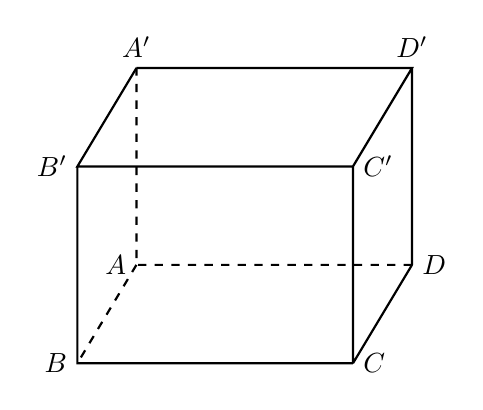
\begin{tikzpicture}[line width=0.8pt, scale=0.5]
		\path
		coordinate (B) at (0,0)
		coordinate (C) at (7,0)
		coordinate (D) at (8.5,2.5)
		coordinate (A) at (1.5,2.5)
		coordinate (B') at (0,5)
		coordinate (C') at (7,5)
		coordinate (D') at (8.5,7.5)
		coordinate (A') at (1.5,7.5)
		;
		\draw [dashed] (D)--(A)--(A') (A)--(B);
		\draw (A')--(B')--(C')--(D')--(A') (C)--(C') (D)--(D') (C)--(D) (C)--(B)--(B');
		\draw (A') node[above] {$A'$};
		\draw (D') node[above] {$D'$};
		\draw (C') node[right] {$C'$};
		\draw (B') node[left]{$B'$};
		\draw (A) node[left] {$A$};
		\draw (D) node[right] {$D$};
		\draw (C) node[right] {$C$};
		\draw (B) node[left] {$B$};
\end{tikzpicture}}
	\loigiai{
		\immini{Ta thấy $\heva{&(ABCD)\parallel (A'B'C'D')\\&(AA'D'D)\parallel (BCC'B')\\&(ABB'A')\parallel (CDD'C')}$ luôn đúng.\\
			và hai mặt phẳng $(BDD'B')$, $(ACC'A')$ là cắt nhau. }{
			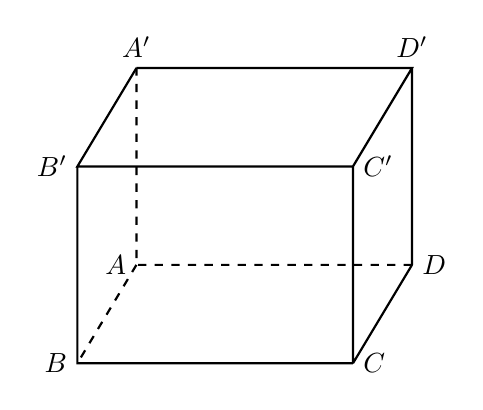
\begin{tikzpicture}[line width=0.8pt, scale=0.5]
				\path
				coordinate (B) at (0,0)
				coordinate (C) at (7,0)
				coordinate (D) at (8.5,2.5)
				coordinate (A) at (1.5,2.5)
				coordinate (B') at (0,5)
				coordinate (C') at (7,5)
				coordinate (D') at (8.5,7.5)
				coordinate (A') at (1.5,7.5)
				;
				\draw [dashed] (D)--(A)--(A') (A)--(B);
				\draw (A')--(B')--(C')--(D')--(A') (C)--(C') (D)--(D') (C)--(D) (C)--(B)--(B');
				\draw (A') node[above] {$A'$};
				\draw (D') node[above] {$D'$};
				\draw (C') node[right] {$C'$};
				\draw (B') node[left]{$B'$};
				\draw (A) node[left] {$A$};
				\draw (D) node[right] {$D$};
				\draw (C) node[right] {$C$};
				\draw (B) node[left] {$B$};
		\end{tikzpicture}}
	}
\end{ex}

\begin{ex}%[1H2B4-2]
	Cho hình chóp $S.ABCD$ có đáy là một hình bình hành. Gọi $A'$, $B'$, $C'$, $D'$ lần lượt là trung điểm của các cạnh $SA,$ $SB,$ $SC,$ $SD.$ Tìm mệnh đề đúng trong các mệnh đề sau.
	\choice
	{$A'C' \parallel BD$}
	{$A'B' \parallel (SAD)$}
	{\True $(A'C'D') \parallel (ABC)$}
	{$A'B' \parallel (SBD)$}
	\loigiai{
		\immini{
			Ta có $A'C'\parallel AC \Rightarrow (A'C'D') \parallel (ABC).$
		}{\begin{tikzpicture}[scale=0.6,every node/.style={scale=0.6}]%hình chóp S.ABCD
				\tkzDefPoints{0/0/A, -2/-2/B, 3/-2/C, -1/4/S}
				\coordinate (D) at ($(A)+(C)-(B)$);
				\tkzDrawSegments[dashed](S,A A,B A,D)
				\tkzDrawPolygon(S,C,D)
				\tkzDefMidPoint(S,A) \tkzGetPoint{A'}
				\tkzDefMidPoint(S,B) \tkzGetPoint{B'}
				\tkzDefMidPoint(S,C) \tkzGetPoint{C'}\\
				\tkzDefMidPoint(S,D) \tkzGetPoint{D'}
				\tkzDrawSegments(S,B B,C)
				\tkzDrawPoints[fill=black](A,B,A',B',C,D,C',D',S)
				\tkzLabelPoints[left](A,B,A',B')
				\tkzLabelPoints[right](C,D,C',D')
				\tkzLabelPoints[above](S)
		\end{tikzpicture}}
	}
\end{ex}

\begin{ex}%[1H2B4-2]
	Cho hình chóp $S.ABCD$, có đáy $ABCD$ là hình bình hành tâm $O$. Gọi $M,N$ lần lượt là trung điểm $SA,SD$. Mặt phẳng $\left(OMN\right)$ song song với mặt phẳng nào sau đây?
	\choice
	{$\left(ABCD\right)$}
	{$\left(SCD\right)$}
	{\True $\left(SBC\right)$}
	{$\left(SAB\right)$}
	\loigiai{
		\immini{
			Vì $ABCD$ là hình bình hành nên $O$ là trung điểm $AC,BD$.\\
			Do đó $MO \parallel SC\Rightarrow MO\parallel \left(SBC\right)$\\
			Và $NO \parallel SB \Rightarrow NO\parallel \left(SBC\right)$\\
			Suy ra $\left(OMN\right)\parallel \left(SBC\right)$.}{\begin{tikzpicture}[line cap=round,line join=round, >=stealth,scale=.7]
				\def \xa{-2}
				\def \xb{-1}
				\def \y{4}
				\def \z{4}
				\coordinate (A) at (0,0);
				\coordinate (B) at ($(A)+(\xa,\xb)$);
				\coordinate (D) at ($(A)+(\y,0)$);
				\coordinate (C) at ($ (B)+(D)-(A) $);
				\coordinate (K) at ($ (A)!1/2!(B) $);
				\coordinate (S) at ($ (K)+(0,\z) $);
				\coordinate (M) at ($ (S)!1/2!(A) $);
				\coordinate (N) at ($ (S)!1/2!(D) $);
				\coordinate (O) at ($ (B)!1/2!(D) $);
				\draw [dashed] (B)--(A)--(D)--(B) (C)--(A)--(S) (O)--(M)--(N)--(O);
				\draw (S)--(B)--(C)--(D)--(S)--(C);
				\tkzDrawPoints(S,A,B,C,D,M,N)
				\tkzLabelPoint[right](D){$ D $}
				\tkzLabelPoints[below right](C)
				\tkzLabelPoints[above](S)
				\tkzLabelPoints[above left](M)
				\tkzLabelPoints[below](O)
				\tkzLabelPoints[above right](N)
				\tkzLabelPoints[above left](A)
				\tkzLabelPoint[below left](B){$ B $}
			\end{tikzpicture}
	}}
\end{ex}

% \centerline{---HẾT---}
\Closesolutionfile{ans}

